\documentclass{article}
\usepackage[T2A]{fontenc}
\usepackage[utf8x]{inputenc}
\usepackage{graphicx}

\usepackage{listings}
\usepackage{xcolor}
\usepackage{tikz}
\usetikzlibrary{calc,shapes.multipart,chains,arrows,positioning}

\tikzset{
    squarecross/.style={
        draw, rectangle,minimum size=18pt, fill=orange!80,
        inner sep=0pt, text=black,
        path picture = {
            \draw[black]
            (path picture bounding box.north west) --
            (path picture bounding box.south east)
            (path picture bounding box.south west) --
            (path picture bounding box.north east);
        }
    }
}

\definecolor{codegreen}{rgb}{0,0.6,0}
\definecolor{codegray}{rgb}{0.5,0.5,0.5}
\definecolor{codepurple}{rgb}{0.58,0,0.82}
\definecolor{backcolour}{rgb}{0.95,0.95,0.92}
\lstdefinestyle{mystyle}{
    backgroundcolor=\color{backcolour},   
    commentstyle=\color{codegreen},
    keywordstyle=\color{magenta},
    numberstyle=\tiny\color{codegray},
    stringstyle=\color{codepurple},
    basicstyle=\ttfamily\footnotesize,
    breakatwhitespace=false,         
    breaklines=true,                 
    captionpos=b,                    
    keepspaces=true,                 
    numbers=left,                    
    numbersep=5pt,                  
    showspaces=false,                
    showstringspaces=false,
    showtabs=false,                  
    tabsize=2
}
\lstset{style=mystyle}

\title{Predator-Prey Model}
\author{ Izmailov Ruslan DS-02 \\ r.izmailov@innopolis.university }
\date{April 2023}

\begin{document}

\maketitle

\textbf{The code of the task, input data and plots available in the github perository: }\\
https://github.com/Hexy00123/PredatorPreyModel/tree/main \\ \\ \\ 

To test this model I used \\
45 victims and 100 killers at the beginning \\ 
$\alpha_1 = 0.3$\\
$\beta_1 = 0.003$\\ 
$\alpha_2 = 0.4$\\ 
$\beta_2 = 0.002$\\ 
Time of simulation = 100\\
Number of time points = 500\\ \\ 
Therefore, input looks like this: \\ 
\texttt{
45 \\
100 \\
0.3 \\ 
0.003 \\ 
0.4 \\ 
0.002 \\ 
100 \\ 
200 \\ 
}

The resulting plots are follows: \\ 
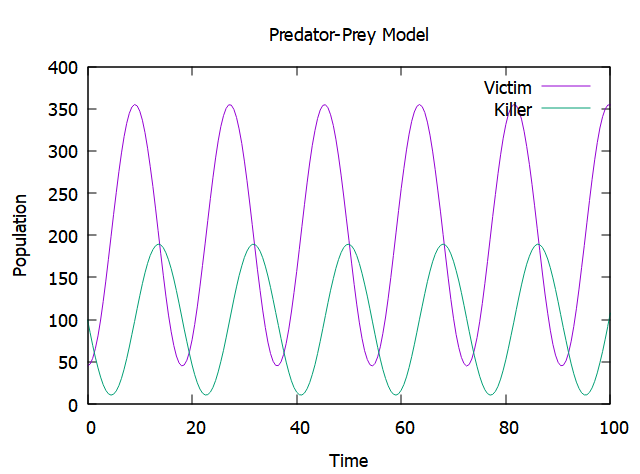
\includegraphics[width=1\linewidth]{PredatorPrey1.png} \\
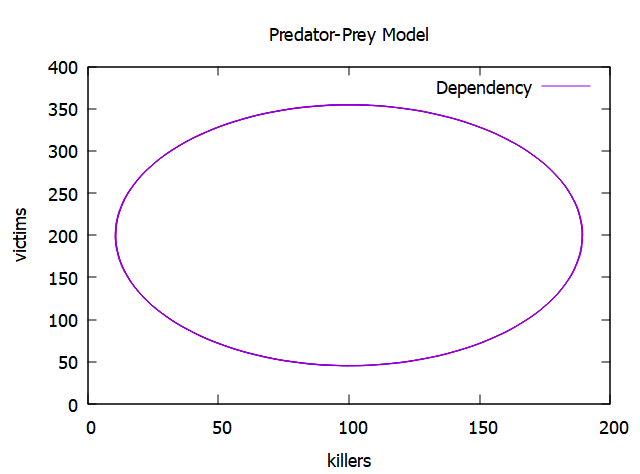
\includegraphics[width=1\linewidth]{PredatorPrey2.png} \\
\newpage
Source code from yandex contest: \\
\begin{lstlisting}[language=C++]
#include <iostream>
#include <vector>
#include <cmath>
#include <iomanip>

using namespace std;

void predatorPrey(int vs, int ks, double a1, double a2, double b1, double b2, int timeLimit, int approximation) {
    /*
     * v'(t) = alpha1 * v(t) + beta1 * v(t) * k(t),
     * k'(t) = -alpha2 * v(t) + beta2 * v(t) * k(t)
     */

    auto time = vector<double>();
    for (double i = 0; i <= timeLimit; i += (double) timeLimit / (double) approximation) {
        time.push_back(i);
    }

    double v0 = vs - a2 / b2;
    double k0 = ks - a1 / b1;

    auto v = vector<double>();
    auto k = vector<double>();
    for (auto t: time) {
        v.push_back(
                v0 * cos(sqrt(a1 * a2) * t) - k0 * sqrt(a2) * b1 * sin(sqrt(a1 * a2) * t) / (b2 * sqrt(a1)) + a2 / b2);

        k.push_back(
                v0 * sqrt(a1) * b2 * sin(sqrt(a1 * a2) * t) / (b1 * sqrt(a2)) + k0 * cos(sqrt(a1 * a2) * t) + a1 / b1);
    }


    cout << "t:\n";
    for (auto value: time)
        cout << value << " ";
    cout << "\n";

    cout << "v:\n";
    for (auto value: v)
        cout << value << " ";
    cout << "\n";

    cout << "k:\n";
    for (auto value: k)
        cout << value << " ";
}


int main() {
    cout << fixed;
    cout << setprecision(2);

    int numberOfVictims, numberOfKillers;
    cin >> numberOfVictims >> numberOfKillers;

    double a1, a2, b1, b2;
    cin >> a1 >> b1 >> a2 >> b2;

    int timeLimit, approximationPoints;
    cin >> timeLimit >> approximationPoints;

    predatorPrey(numberOfVictims, numberOfKillers, a1, a2, b1, b2, timeLimit, approximationPoints);
    return 0;
}
\end{lstlisting} \\ 

Source code for plotting: \\ 
\begin{lstlisting}[language=C++]
#include <iostream>
#include <vector>
#include <cmath>
#include <iomanip>

using namespace std;

vector<vector<double>>
predatorPrey(int vs, int ks, double a1, double a2, double b1, double b2, int timeLimit, int approximation) {
    /*
     * v'(t) = alpha1 * v(t) + beta1 * v(t) * k(t),
     * k'(t) = -alpha2 * v(t) + beta2 * v(t) * k(t)
     */

    auto time = vector<double>();
    for (double i = 0; i <= timeLimit; i += (double) timeLimit / (double) approximation) {
        time.push_back(i);
    }

    double v0 = vs - a2 / b2;
    double k0 = ks - a1 / b1;

    auto v = vector<double>();
    auto k = vector<double>();
    for (auto t: time) {
        v.push_back(
                v0 * cos(sqrt(a1 * a2) * t) - k0 * sqrt(a2) * b1 * sin(sqrt(a1 * a2) * t) / (b2 * sqrt(a1)) + a2 / b2);

        k.push_back(
                v0 * sqrt(a1) * b2 * sin(sqrt(a1 * a2) * t) / (b1 * sqrt(a2)) + k0 * cos(sqrt(a1 * a2) * t) + a1 / b1);
    }

    auto res = vector<vector<double>>();
    res.push_back(time);
    res.push_back(v);
    res.push_back(k);
    return res;
}

#ifdef WIN32
#define GNUPLOT_NAME "C:\\gnuplot\\bin\\gnuplot -persist"
#else
#define GNUPLOT_NAME "gnuplot -persist"
#endif

int main() {
#ifdef WIN32
    FILE *victimsAndKillersOfTime = _popen(GNUPLOT_NAME, "w");
    FILE *victimsOfKillers = _popen(GNUPLOT_NAME, "w");
#else
    FILE* victimsAndKillersOfTime = popen(GNUPLOT_NAME, "w");
    FILE *victimsOfKillers = _popen(GNUPLOT_NAME, "w");
#endif

    cout << fixed;
    cout << setprecision(2);

    int numberOfVictims, numberOfKillers;
    cin >> numberOfVictims >> numberOfKillers;

    double a1, a2, b1, b2;
    cin >> a1 >> b1 >> a2 >> b2;

    int timeLimit, approximationPoints;
    cin >> timeLimit >> approximationPoints;

    auto res = predatorPrey(numberOfVictims, numberOfKillers, a1, a2, b1, b2, timeLimit, approximationPoints);
    auto t = res[0], v = res[1], k = res[2];

    fprintf(victimsAndKillersOfTime, "set title 'Predator-Prey Model'\n");
    fprintf(victimsAndKillersOfTime, "set xlabel 'Time'\n");
    fprintf(victimsAndKillersOfTime, "set ylabel 'Population'\n");
    fprintf(victimsAndKillersOfTime,
            "plot '-' using 1:2 with lines title 'Victim', '-' using 1:2 with lines title 'Killer'\n");

    fprintf(victimsOfKillers, "set title 'Predator-Prey Model'\n");
    fprintf(victimsOfKillers, "set xlabel 'killers'\n");
    fprintf(victimsOfKillers, "set ylabel 'victims'\n");
    fprintf(victimsOfKillers,
            "plot '-' using 1:2 with lines title 'Dependency', '-' using 1:2 with lines title 'Predator'\n");

    // Plot the prey and predator populations
    for (int i = 0; i < t.size(); ++i)
        fprintf(victimsAndKillersOfTime, "%f\t%f\n", t[i], v[i]);
    fprintf(victimsAndKillersOfTime, "e\n");

    for (int i = 0; i < t.size(); ++i)
        fprintf(victimsAndKillersOfTime, "%f\t%f\n", t[i], k[i]);
    fprintf(victimsAndKillersOfTime, "e\n");

    for (int i = 0; i < t.size(); ++i) {
        fprintf(victimsOfKillers, "%f\t%f\n", k[i], v[i]);
    }
    fprintf(victimsOfKillers, "e\n");

    fflush(victimsAndKillersOfTime);
    fflush(victimsOfKillers);
#ifdef WIN32
    _pclose(victimsAndKillersOfTime);
    _pclose(victimsOfKillers);
#else
    pclose(victimsAndKillersOfTime);
    pclose(victimsOfKillers);
#endif

    return 0;
}

\end{lstlisting}






\end{document}
